\documentclass[10pt]{beamer}
\mode<presentation> {
	%\usetheme{AnnArbor}
	%\usetheme{Antibes}
	%\usetheme{CambridgeUS}
	%\usetheme{Copenhagen}
	%\usetheme{Darmstadt}
	\usetheme{Dresden}
	%\usetheme{Frankfurt}
	%\usetheme{Goettingen}
	%\usetheme{Hannover}
	%\usetheme{Ilmenau}
	%\usetheme{JuanLesPins}
	%\usetheme{Luebeck}
	%\usetheme{Madrid}
	%\usetheme{Marburg}
	%\usetheme{Montpellier}
	%\usetheme{PaloAlto}
	%\usetheme{Singapore}
	%\usetheme{Warsaw}
	%\usecolortheme{beaver}
	%\usecolortheme{crane}
	\usefonttheme[onlymath]{serif}
}

\usepackage{graphicx} % Allows including images
\usepackage{booktabs, setspace, amsfonts} % Allows the use of \toprule, \midrule and
\usepackage{CJKutf8, indentfirst, ulem, url}
\usepackage{amsmath, multirow}

\setlength{\parskip}{1em}

\begin{document}
\begin{CJK}{UTF8}{gkai}
	\begin{spacing}{1.2}

		\title[计算几何]{计算几何} % The short title appears at the bottom of every slide, the full title is only on the title page

		\author{Hometown} % Your name
		\institute[雅礼中学] % Your institution as it will appear on the bottom of every slide, may be shorthand to save space
		{
			雅礼中学\medskip
		}
		\date{\today} % Date, can be changed to a custom date

		\begin{frame}
			\titlepage % Print the title page as the first slide
		\end{frame}
		\section{Preface}
		\begin{frame}

			今天讲课大概是两个部分,一个是计算几何的基础知识,另一个就是相关的一些算法。 \pause

			关于计算几何的基础知识,我只会讲几个比较常用的或者难的函数。其余的一些函数大家可以课后去看基础模板的代码。

		\end{frame}
		\section{Basic Knowledge}
		\subsection{Vector}
		\begin{frame}
			\frametitle{向量的基本运算}

			一般来说,在计算几何中,我们更习惯于用向量的坐标表示,即用$(x,y)$来表示一个以$(0,0)$为起点,$(x,y)$为终点的一个向量。 \pause

			向量的加减,直接两维坐标相加减即可。向量与标量乘除,直接两维坐标做乘除就好了。

		\end{frame}
		\begin{frame}
			\frametitle{向量的点积}

			$a \cdot b = |a||b| \cos \theta$,其中$\theta$表示向量$a$旋转到向量$b$经过的夹角。点积的绝对值等于$a$向量在$b$向量上的投影的模长与$b$向量模长的乘积。(好像没什么用) \pause

			当我们以坐标形式表示向量时,设 $a = (x_1,y_1),b = (x_2,y_2)$,则有 $a \cdot b = x_1x_2 + y_1y_2$。

		\end{frame}
		\begin{frame}
			\frametitle{向量的叉积}

			$a \times b = |a||b| \sin \theta$,其中 $\theta$ 表示向量 $a$ 旋转到向量 $b$ 经过的夹角。叉积的几何意义表示的是以这两个向量为邻边构成的平行四边形的面积。其中当 $\theta > 0$ 时为正,$\theta < 0$ 时为负。 \pause

			当我们以坐标形式表示向量时,设 $a=(x_1,y_1),b=(x_2,y_2)$,则有 $a \times b = x_1y_2-x_2y_1$。 \pause

			向量叉积可以用来判断向量的方向。对于两个向量 $a,b$,若 $a \times b > 0$,则当我们把两个向量平移,使他们共起点时,$b$ 在 $a$ 的逆时针方向。

		\end{frame}
		\begin{frame}
			\frametitle{向量的旋转}

			把向量 $a=(x,y)$ 逆时针旋转 $\theta$,得到的向量为 $$a'=(x \cos \theta - y \sin \theta,x \sin \theta + y \cos \theta)$$ \pause
			证明可以考虑设原向量与 $x$ 轴正方向的夹角,然后利用和角公式计算。 \pause
			
			设 $a$ 与 $x$ 轴正方向夹角为 $\alpha$,则有 $x = |a| \cos \alpha,y = |a| \sin \alpha$。旋转后所求即为 $(|a| \cos(\alpha + \theta) , |a| \sin(\alpha + \theta))$,带入计算即可。

		\end{frame}
		\subsection{Line}
		\begin{frame}
			\frametitle{直线的表示方式}

			计算几何中,直线一般有两种表示方式。一种是用两个点来表示,另一种是用一个点和一个从这个点出发的向量表示(好像没什么区别……) \pause

			利用第二种表达方式,我们甚至可以表示一个半平面。即设这个向量的左边为表示的半平面。

		\end{frame}
		\begin{frame}
			\frametitle{点到直线与点到线段距离}

			在使用上面所说的直线表示方式的情况下,点到直线距离公式再使用解析几何中的东西似乎就不那么方便了。 \pause 我们考虑用叉积的形式。考虑两个向量的叉积的几何意义指的是两个向量为邻边形成的平行四边形的有向面积,因此用面积除以底边长即可。 \pause

			点到线段距离是一样的,判断一下几种情况即可。

		\end{frame}
		\begin{frame}
			\frametitle{点到直线的投影}
			\begin{center}
			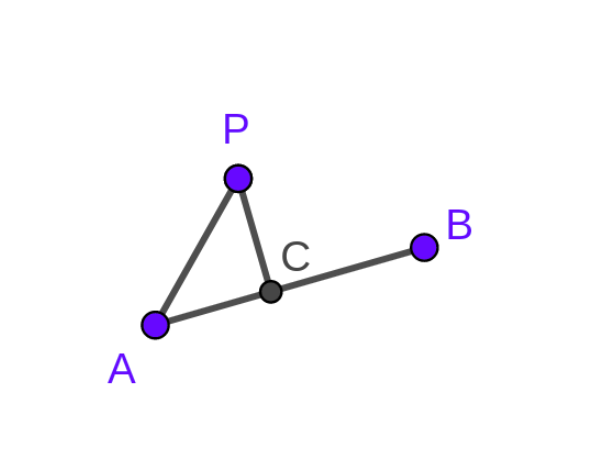
\includegraphics[scale=0.18]{../Pictures/Line_Projection.png}
			\end{center}

			首先可以求出向量 $\overrightarrow{AP} \cdot \overrightarrow{AB} = |AC||AB|$ 和 $\overrightarrow{AB} \cdot \overrightarrow{AB} = |AB||AB|$。于是就可以求出 $\frac{|AC|}{|AB|}$。这样$C = A + \overrightarrow{AB} \times \frac{|AB|}{|AC|}$。
		\end{frame}
		\begin{frame}
			\frametitle{两直线的交点与相交判定}
			\begin{center}
			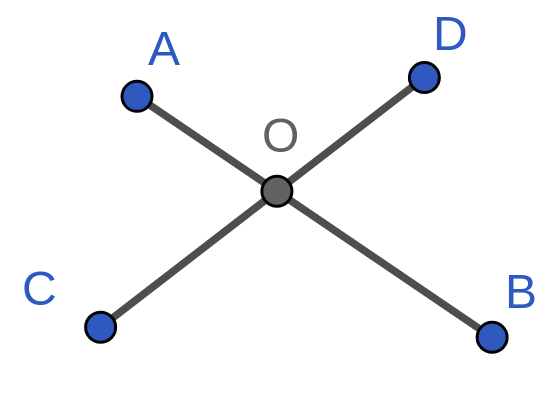
\includegraphics[scale=0.14]{../Pictures/Line_Intersection.png}
			\end{center}
			求交点常用的方法同样是利用叉积。我们可以先求出 $\triangle ABC$ 和 $\triangle ABD$ 的面积,从而得到 $OC$ 与 $OD$ 的比值。然后就可以得到 $O$ 点坐标了。 \pause

			对于相交判定,先考虑直线与线段的相交判定,利用叉积判断线段两点是否在直线的同侧即可。 \pause 对于线段与线段判交,分别做两次直线与线段判交即可。

		\end{frame}
		\subsection{Circle And Polygon}
		\begin{frame}
			\frametitle{圆与圆交点}
			这里只考虑两圆相交的情况,其余情况都比这个简单吧…… \pause
			\begin{center}
			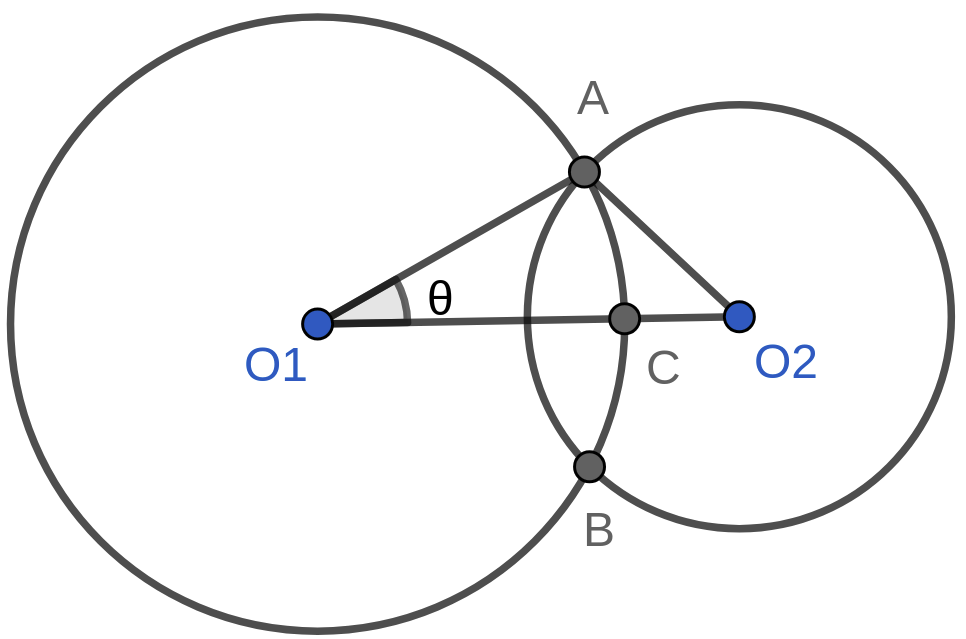
\includegraphics[scale=0.14]{../Pictures/Circle_Intersection.png}
			\end{center}
			如图,首先可以由余弦定理,求出 $\theta = \angle AO_1O_2$。将向量 $\overrightarrow{O_1C}$ 旋转 $\theta$ 即可得到一个交点,另一个交点同理可得。

		\end{frame}
		\begin{frame}
			\frametitle{点到圆的切线}
			\begin{center}
			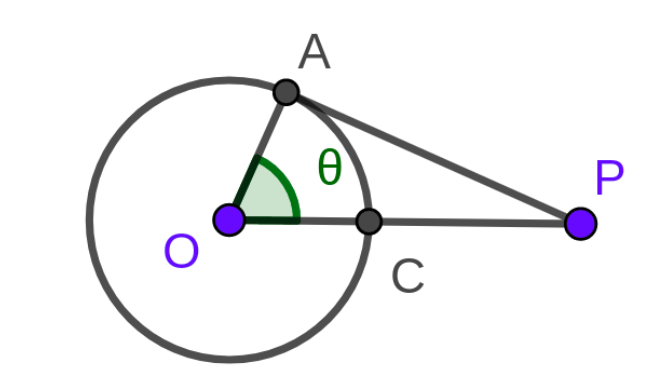
\includegraphics[scale=0.14]{../Pictures/Tangent_Line_Through_Point.png}
			\end{center}
			首先求出 $\theta = \angle AOP$。然后把向量 $\overrightarrow{OC}$ 旋转 $\theta$ 即可求出两个交点。

		\end{frame}
		\begin{frame}
			\frametitle{两圆的公切线}
			先考虑外公切线,内公切线同理可得。 \pause
			\begin{center}
			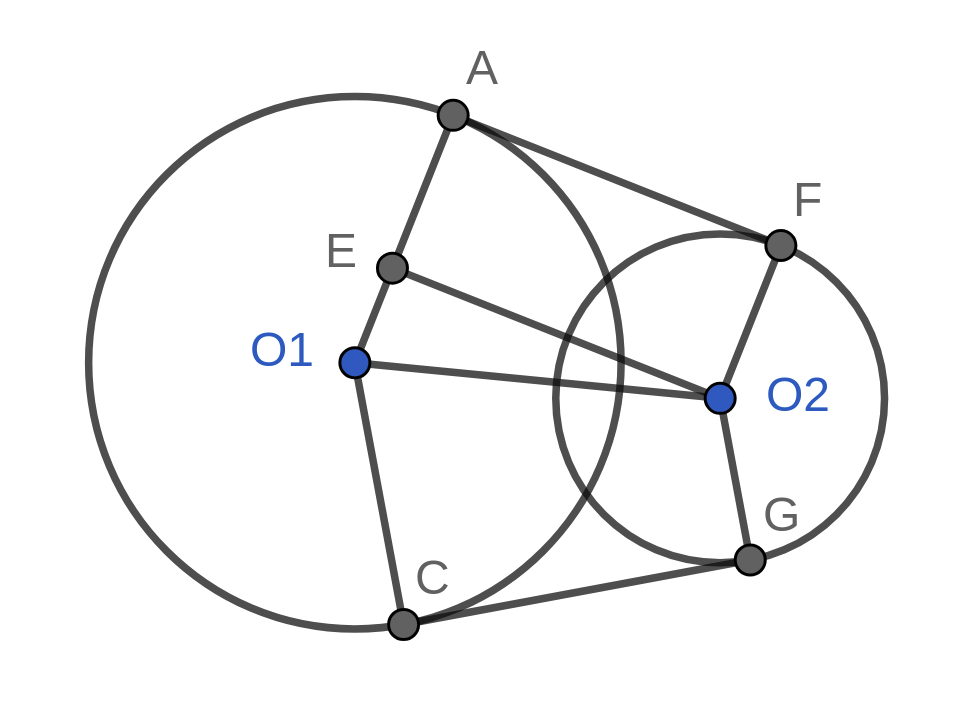
\includegraphics[scale=0.14]{../Pictures/Tangent_Line.png}
			\end{center}
			如图,不难求出 $\mathrm{Rt}\triangle EO_1O_2$ 各边长,所以亦可以求出 $\angle EO_1O_2$。于是又可以求出向量 $O_1A$ 的极角,从而出 $A$ 点坐标,$F$ 点坐标类似。

		\end{frame}
		\begin{frame}
			\frametitle{判断点在多边形内}

			假想有一条从该点出发,水平向右的射线。依次枚举多边形相邻两点,统计这两个点的连边穿过这条射线的次数。若逆时针穿过,则计数器 $+1$,顺时针穿过时,计数器 $-1$ 。 \pause

			如果计数器为 $0$,则点在多边形外部,否则在多边形内部。
			
			注意判断点在多边形上的情况。

		\end{frame}
		\section{Basic Algorithms And Problems}
		\subsection{Convex Hull}
		\begin{frame}
			\frametitle{凸包}

			相信大家都知道凸包是干什么的。 \pause

			实现起来很简单。把所有点按照 $x$ 坐标排序,用栈记录当前在凸包内的点。依次检查保证斜率的单调性,正反各做一次。检查斜率单调性的时候,使用叉积判断两向量的相对位置即可。

		\end{frame}
		\begin{frame}
			\frametitle{UVA11168 Airport}

			给定一个大小为 $n$ 的点集,你需要做一条直线,满足所有点在直线的同侧(可以在直线上),并最小化所有点到这条直线的距离的平均值。只需输出这个距离平均值即可。 \pause

			$n \le 10000$,数据组数 $T \le 65$。

		\end{frame}
		\begin{frame}
			\frametitle{UVA11168 Solution}

			首先可以发现,直线是不能穿过这 $n$ 个点的凸包的,于是满足要求的直线一定在凸包的某条边上。为何这条直线不会只过凸包的一个点呢? \pause

			证明可以考虑设一个关于直线倾斜角的函数。求导之后发现导数一定是单调递减的。因此极值点只会出现在定义域的两端。接下来的问题就是,如何快速求 $n$ 个点到一条直线的距离之和? \pause

			这个问题用向量似乎不那么好解决,于是考虑用解析几何的方法。\pause 我们知道点到直线的距离满足 $d = \frac{|Ax_0+By_0+C|}{\sqrt{A^2 + B^2}}$,由于所有点一定在这条直线的同侧,因此绝对值可以去掉,最后求完和统一做一个绝对值。剩下的只要预处理出所有点的横纵坐标之和,就可以在 $O(1)$ 的时间内求出一条直线的答案。总时间复杂度 $O(Tn)$。

		\end{frame}
		\begin{frame}
			\frametitle{BZOJ4570 [SCOI2016]妖怪}

			邱老师共有 $n$ 只妖怪,每只妖怪有攻击力和防御力两种属性。

			在某种环境 $(a,b)$ 中,妖怪可以降低自己 $ka$ 点攻击力,提升 $kb$ 点防御力。其中 $a,b$ 属于实数,$k$ 为任意实数,但是两种属性必须始终非负。注意 $a,b$ 可以为负数。

			妖怪在环境 $(a,b)$ 中的战斗力为妖怪在该环境中能达到最大攻击力和最大防御力之和,即 $val(a,b) = \max(atk(a,b)) + \max(dnf(a,b))$。给定每只妖怪的两种属性的初始值,求在环境最不利的环境下,战斗力最强的妖怪的战斗力。 \pause

			$n \le 10^6$。

		\end{frame}
		\begin{frame}
			\frametitle{BZOJ4570 Solution}

			首先,一个很显然的性质,如果把一只妖怪的两个属性看做二维平面上的一个点,那么在某一环境下妖怪的战斗力,也就是过这个点的某一条直线与 $x$ 轴和 $y$ 轴交点坐标之和。 \pause

			于是题目所求就可以转化为,给定二位平面内的 $n$ 个点,确定一个直线的斜率,使得分别过这 $n$ 个点的 $n$ 条直线的横纵坐标之和最大的直线尽可能小。 \pause

			于是我们可以先求出凸包,那么对答案造成贡献的点一定在凸包上。注意到横纵坐标之和是一个和斜率有关的对勾函数。于是我们分类讨论出函数的最小值即可。时间复杂度 $O(n \log n)$。

		\end{frame}
		\begin{frame}
			\frametitle{清橙1279 集合的面积}

			给定两个点集 $A,B$,定义两个点 $a,b$ 的加法 $a(x_1,y_1) + b(x_2,y_2) = (x_1 + x_2,y_1 + y_2)$。定义两个点集的加法 $A + B = \{a + b| a \in A, b \in B\}$(即闵可夫斯基和),求点集 $A + B$ 的凸包的面积。

			$|A|, |B| \le 10^5$,坐标范围不超过 $10^8$。

		\end{frame}
		\begin{frame}
			\frametitle{清橙1279 Solution}

			考虑点集 $A + B$ 的凸包上的每一个点 $c = a + b$,那么 $a$ 一定位于 $A$ 的凸包上,$b$ 一定位于 $B$ 的凸包上。 \pause

			这样这个凸包可以看做是 $A$ 凸包上一个定点在 $B$ 凸包上转一圈,所有点出现过的位置的集合。 \pause
			
			仔细分析这个转一圈的过程,我们发现 $A + B$ 的凸包就是 $A$ 的凸包的边和 $B$ 的凸包的边按极角排序后首尾相连所得图形。

		\end{frame}
		\begin{frame}
			\frametitle{动态凸包}

			\pause
			动态凸包支持以下几个操作:
			\begin{itemize}
				\item 查询面积 $O(1)$
				\item 动态插入 均摊 $O(\log n)$
				\item 查询某个点是否在凸包内 $O(\log n)$
			\end{itemize}
			\pause
			具体做法就是上凸壳与下凸壳各维护一个以 $x$ 坐标为键值的 \texttt{std::set}。然后首先在 \texttt{set} 上找到点的位置。然后用叉积判一下新加的点是否在凸包内。然后依次向左向右删除需要删除的点即可。顺便维护一下凸包的面积。 \pause

			模板题可以看看 Codeforces 70D。

		\end{frame}
		\subsection{Rotating Calipers}
		\begin{frame}
			\frametitle{旋转卡壳}

			旋转卡壳,顾名思义,就是两条平行的直线卡在凸包的两边,绕着凸包旋转一圈,对于每一对直线上一起出现过的点对距离长度取最大值,从而得到凸包的直径这样一个过程。其中这个点对被称为对踵点。 \pause

			首先,为什么这么求出来就是凸包的直径? \pause 考虑一个凸包的直径,如果它的两个端点不是一对对踵点,那么一定存在一对新的対踵点,满足这两个点的距离大于当前考虑的两个点。

		\end{frame}
		\begin{frame}
			\frametitle{旋转卡壳}

			似乎到这里代码上还是不太好实现,怎么模拟平行线绕凸包旋转的过程呢? \pause

			这里只要拿两个指针,分别表示扫到当前状态的对踵点。然后每次先移动其中一个指针,然后看第二个指针要移到什么地方,依次取最大值即可。 \pause

			容易发现,这个过程中也可以求出到凸包上的每一条边距离最远的点。

		\end{frame}
		\begin{frame}
			\frametitle{BZOJ1069 [SCOI2007]最大土地面积}

			给定 $n$ 个点的坐标,从中选择 $4$ 个点,最大化这 $4$ 个点组成的四边形的面积。 \pause

			$n \le 2000$。

		\end{frame}
		\begin{frame}
			\frametitle{BZOJ1069 Solution}

			首先不难证明四个点一定都在凸包上。考虑枚举四边形的对角线,这样我们只要最大化对角线两边的三角形面积即可。这个只需要在枚举第二个点的过程中,顺便做旋转卡壳求出两边距离最远的点即可。 \pause

			时间复杂度 $O(n^2)$。

		\end{frame}
		\begin{frame}
			\frametitle{清橙1334 最远点}

			给你一个 $n$ 个点的凸多边形,求离每一个点最远的点。

			$n \le 500000$。

		\end{frame}
		\begin{frame}
			\frametitle{清橙1334 Solution}

			需要注意的是,旋转卡壳并不能求出距离每个点最远的点。 \pause

			容易发现距离一个点的最远点,是决策单调的。因此只需要利用决策单调性,用队列维护决策点就行了。

		\end{frame}
		\begin{frame}
			\frametitle{[Codeplus 5] 法师}

			给出 $n$ 个点,两两连边,以每一条边为直径作圆,求圆的并的周长。

			$n \le 10^5$。

		\end{frame}
		\begin{frame}
			\frametitle{[Codeplus 5] 法师 Solution}

			考虑一个点位于这些圆的并之中需要满足什么条件。某个点处于这些圆的并之中,当且仅当这个点可以找到一条直径,使得这个点张这条直径的张角 $\ge 90$°。 \pause

			于是可行区域的边界可以视为,使用一个直角去卡这个点集,然后在直角旋转过程中,端点留下的路径,答案就是这个直角的顶点的轨迹长度。容易发现只需保留凸包上的点即可。 \pause

			这个过程容易让人想到旋转卡壳。类似与旋转卡壳,这样合法的直径条数是 $O(n)$ 级别的。于是旋转卡壳的时候,求出每个圆弧的角度大小即可。这个求每个圆弧角度的过程大概用个圆的交点什么的就行了。

		\end{frame}
		\subsection{Half-plane Intersection}
		\begin{frame}
			\frametitle{半平面交}

			类似于凸包的做法,和凸包又有所不同。按照之前所说的,直线可以表示一个半平面,先将所有半平面按照对应直线极角来排序,按照顺序加入一个双端队列。每次新加入一个半平面,就判断一下队首两个半平面的交点,队尾两个半平面的交点,与新的半平面的位置关系,前后弹队列。最后注意两个边界: \pause
			\begin{itemize}
				\item 当两个半平面的极角相同的时候,需要取更靠左的那一个。 \pause
				\item 最后收尾的时候,可能第一个半平面还有可能把最后的半平面排除掉,因此最后还要弹一次队列。
			\end{itemize}

		\end{frame}
		\begin{frame}
			\frametitle{LA4992 Jungle Outpost}

			在丛林中有 $n$ 个眺望台,形成一个凸 $n$ 边形。这些眺望台的保护范围就是这个凸多边形内的任意点。敌人进攻时,会炸毁一些眺望台,使得总部暴露在那些剩下的眺望台的凸包之外。你的任务是选择一个点作为总部,使得敌人需要炸坏的眺望台数量尽可能多。注意敌人炸毁眺望台的时候,敌人已经知道你总部的位置 \pause

			$n \le 50000$。

		\end{frame}
		\begin{frame}
			\frametitle{LA4992 Solution}

			首先考虑敌人的最优策略是什么。\pause 敌人肯定会炸毁相邻的眺望台。炸毁了相邻眺望台之后,还未被暴露的区域就是一个个半平面。 $n$ 种炸毁的方法对应 $n$ 个半平面,如果存在一个合法的总部,等价于这 $n$ 个半平面的半平面交是存在的。\pause

			因此我们二分答案,然后每次检查的时候就用半平面交判断是否存在。时间复杂度 $O(n \log^2 n)$。

		\end{frame}
		\begin{frame}
			\frametitle{UOJ242 [UR 16]破坏蛋糕}
			
			平面上有 $n + 1$ 条直线,前 $n$ 条直线把平面分成许多块,这些块有些面积有限,有些面积无限,而第 $n + 1$ 条直线不经过前 $n$ 条直线的交点,且一定不和前 $n$ 条直线中的任意一条平行,求第 $n + 1$ 条直线被前 $n$ 条直线划分成的 $n + 1$ 段中哪些在面积有限的块里,哪些在面积无限的块里。按照从左到右的顺序输出每个区域的情况。 \pause

			$n \le 10^5$。保证第 $n + 1$ 条直线不与 $x$ 轴垂直。

		\end{frame}
		\begin{frame}
			\frametitle{UOJ242 Solution}

			这题放半平面交里可能有点牵强,但是又和半平面交有点关系…… \pause

			首先考虑 $O(n^2 \log n)$ 的暴力该怎么做。 \pause对于每一段,我们分别取一个关键点(例如中点),我们只需要判断这个点所在的区域是否为无限即可。不难发现我们只要对每个区域做一次半平面交就可以了。具体来说,每个半平面指的是,对于每一条直线,关键点所在的那一侧的区域。事实上,求半平面交的地方是可以简化的,只需要按照极角排好序之后,相邻两个向量的差均小于 $\pi$,这个区域就是有限的。 \pause

			怎么优化到 $O(n^2)$ 呢?\pause 首先上述算法的瓶颈在于排序。注意到从第 $i$ 段到第 $i + 1$ 段,只会有一个向量改变方向,因此排序的过程也就可以略去了。

		\end{frame}
		\begin{frame}
			\frametitle{UOJ242 Solution}

			相信优化到这里的时候,大家都会做了。用一个 \texttt{std::set} 来维护每个向量的极角,每次更新一下计数器就可以了。 \pause

			时间复杂度$O(n \log n)$。 \pause

			这个题有点卡精度,eps要设小一点。

		\end{frame}
		\section{More Algorithms}
		\subsection{Inversive Geometry}
		\begin{frame}
			\frametitle{圆的反演}
			
			首先给出圆的反演的定义。

			已知一圆 $C$,圆心为 $O$,半径为 $r$,如果 $P$ 与 $P’$ 在过圆心 $O$ 的直线上,且$|OP||OP'| = r^2$,则称 $P$ 与 $P'$ 关于 $O$ 互为反演。 \pause

			这个定义有点圆幂的感觉,所以后面许多证明与相似三角形相关。 \pause

			一个显然的性质就是,除反演中心外,平面上的每一个点都只有唯一的反演点,且这种关系是对称的,位于反演圆上的点,保持在原处,位于反演圆外部的点,变为圆内部的点,位于反演圆内部的点,变为圆外部的点。

		\end{frame}
		\begin{frame}
			\frametitle{圆的反演的一些性质}

			任意一条不过反演中心的直线,它的反形是经过反演中心的圆,反之亦然,特别地,过反演中心相交的圆,变为不过反演中心的相交直线。 \pause

			\begin{center}
			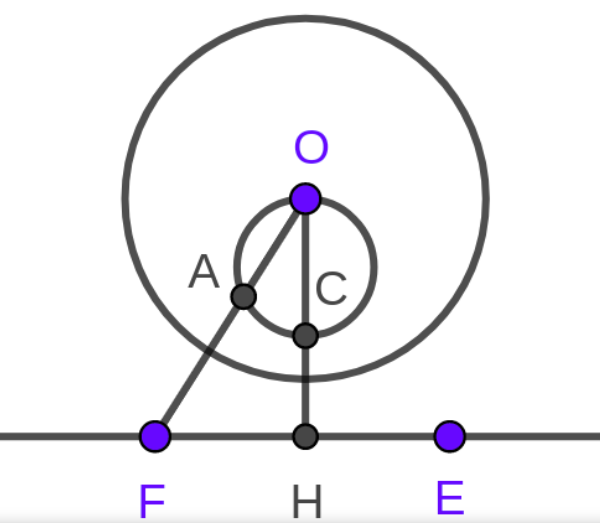
\includegraphics[scale=0.14]{../Pictures/Circle_Inversion_1.png}
			\end{center}

			至于证明,可以很容易发现利用相似三角形就可以证明了。

		\end{frame}
		\begin{frame}
			\frametitle{圆的反演的一些性质}

			不过反演中心的圆,它的反形是一个圆,反演中心是这两个互为反形的圆的一个位似中心,任意一对反演点是逆对应点。 \pause

			\begin{center}
			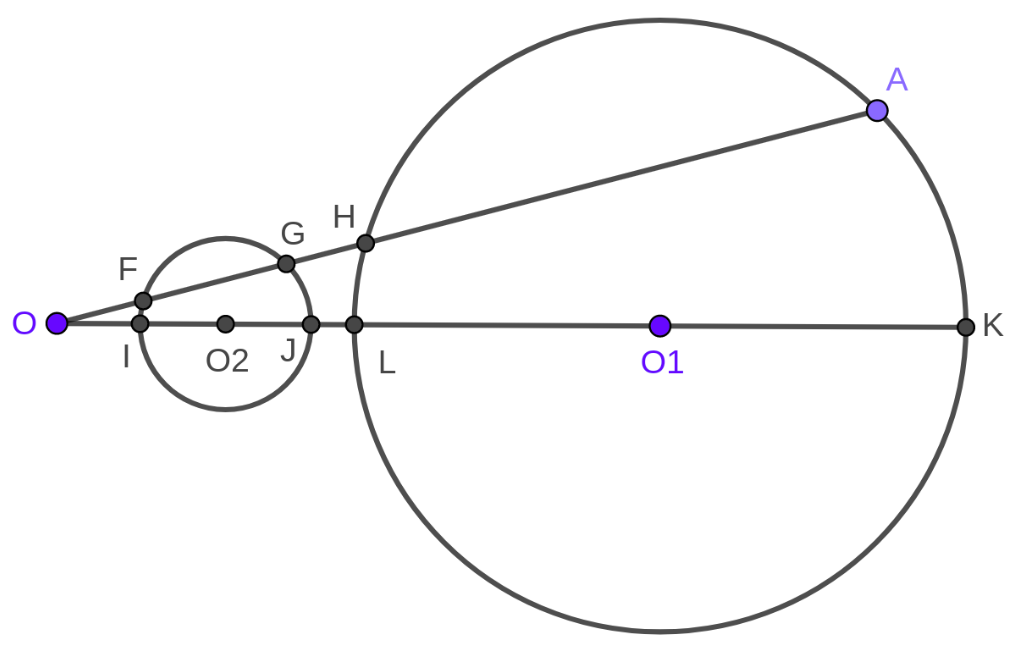
\includegraphics[scale=0.14]{../Pictures/Circle_Inversion_2.png}
			\end{center}

			只需证明 $\triangle OIG \sim \triangle OHK,\triangle OGJ \sim \triangle OLH$ 即可得 $\angle IGJ = 90$°

		\end{frame}
		\begin{frame}
			\frametitle{圆的反演的实现}

			容易发现,对于第一种情况,求出反演后的图形是比较容易的。难点在于第二种情况。 \pause

			对于上图中圆 $O$ 的半径为 $r$,圆 $O_1$ 的半径为 $r_1$,圆 $O_2$ 的半径为 $r_2$,则有。
			\begin{align}
				OJ \cdot OL = (OO_2 + r_2)(OO_1 - r_1) = r^2 \notag \\
				OI \cdot OK = (OO_2 - r_2)(OO_1 + r_1) = r^2 \notag
			\end{align}

			解得 $r_2 = \frac{1}{2}(\frac{1}{OO_2 - r_1} - \frac{1}{OO_2 + r_1}) r^2$ \pause 。再利用 $O$ 和 $O_1$ 的坐标,$O_2$坐标也很容易得到了。
		\end{frame}
		\begin{frame}
			\frametitle{HDU4773}

			讲了这么多,这玩意儿到底能干啥呢?来看一个简单的题目。 \pause

			给定两个相离的圆的半径和圆心,在这两个圆外给定一个点 $P$,求过点 $P$ 的圆且与已知的两个圆外切的所有圆的总数和它们的圆心坐标和半径。

		\end{frame}
		\begin{frame}
			\frametitle{HDU4773 Solution}

			这个东西直接计算几何强算似乎很不好算。于是考虑利用圆反演。 \pause

			先以点 $P$ 为为反演中心,反演半径为 $1$,把圆 $C_1$ 和圆 $C_2$ 反演后再求这两个圆的公切线,再把这个公切线反演回去,那么就是一个过点 $P$ 的圆,且与原来的 $C_1$ 和 $C_2$ 相切。 \pause

			两圆公切线的求法之前已经讲过了。这里就利用反演将圆转化为直线,用直线来解决有些圆不好解决的问题。

		\end{frame}

		\subsection{Minimum Covered Circle}
		\begin{frame}
			\frametitle{最小圆覆盖}

			最小圆覆盖可以在 $O(n)$ 的时间内求出覆盖 $n$ 个点的最小的圆。 \pause

			解决最小圆覆盖问题通常使用随机增量法。

		\end{frame}
		\begin{frame}
			\frametitle{最小圆覆盖}

			把点的顺序随机打乱后依次加入,加入点 $i$ 时,若点 $i$ 不在前 $i-1$ 个点的最小覆盖圆内,说明它在新圆的边界上,那么变成下面的子问题。
			
			已知点 $i$ 在圆的边界上,求前 $i$ 个点的最小覆盖圆。依次加入每个点,加到点 $j$ 时如果 $j$ 不在前 $j - 1$ 个点和点 $i$ 的最小覆盖圆内,说明它在新圆的边界上,同样会变成一个子问题。

			已知点 $i,j$ 在圆的边界上,求前 $j$ 个点和点 $i$ 的最小覆盖圆。依次加入每个点,加到点 $k$ 时如果 $k$ 不在前 $k-1$ 个点和点 $i$ 及点 $j$ 的最小覆盖圆内,说明最小覆盖圆上的三个点就是 $i,j,k$ 了。

		\end{frame}
		\begin{frame}
			\frametitle{最小圆覆盖}

			来分析一下时间复杂度。\pause

			最底层的子问题复杂度显然是 $O(n)$ 的。\pause

			对于第二层的子问题,当枚举到 $j$ 时会有 $\frac{3}{j}$ 的概率需要做一遍 $O(j)$ 的下一个子问题,因此复杂度是 $O(n)$ 的。\pause

			同理可得第一层也是 $O(n)$ 的。这样我们就得到了一个优秀的线性做法。

		\end{frame}
		\subsection{Scanline}
		\begin{frame}
			\frametitle{扫描线}

			一般来说,扫描线在计算几何中的常见做法,即扫描线扫过去的时候,用数据结构或者直接暴力维护扫描线上的信息并统计答案。\pause

			似乎没什么好说的……直接来看题。

		\end{frame}
		\begin{frame}
			\frametitle{HDU1542 Atlantis}

			给定 $n$ 个矩形,求矩形的并的面积。 \pause

			原题 $n \le 100$,这里假装 $n \le 10^5$ 好了。

		\end{frame}
		\begin{frame}
			\frametitle{HDU1542 Solution}

			先离散化,然后扫描线从小到大扫描,用线段树维护扫描线的信息。线段树里维护两个tag,一个是这个区间被覆盖的次数,另一个是这个区间内有多少个点被覆盖了。 \pause

			第一个tag在维护的时候不要push\_down,便于维护第二个tag。第二个tag在维护的时候,分情况讨论一下: \pause

			如果这个区间的第一个tag不为 $0$,那么第二个tag的值为区间的长度,否则第二个tag的值为左右儿子的tag值相加。由于我们维护的时候是从下往上传上来的,因此这样维护是正确的。

		\end{frame}
		\begin{frame}
			\frametitle{LOJ6260 [Codeplus2] 寄蒜几盒}

			在二维平面上有 $n$ 条直线,这些直线会将平面划分成若干个区域。给定 $m$ 个点,求每个点所在的区域的面积。

			保证询问的点与直线的距离大于 $10^{-7}$。

			$n \le 500,m \le 100000$。

		\end{frame}
		\begin{frame}
			\frametitle{LOJ6260 Solution}

			首先离线询问,并对直线两两求交。然后用一条扫描线从左到右扫过去,维护每一条直线的高低关系。每次到了一个交点就交换两条直线的高低关系。扫到一个询问之后,就在这些直线中二分得到当前的区域。 \pause

			为了计算面积,我们还需要在某个区域遇到一个交点的时候,重新维护一下当前区域的面积,这个可以直接用叉积计算。

		\end{frame}
		\subsection{Simpson's rule}
		\begin{frame}
			\frametitle{辛普森积分}

			对于二次曲线求积分的时候,我们可以用一个这样的式子来求: \pause
			$$ \int_{L}^{R} f(x)\,dx = \frac{R - L}{6}[f(L) + f(R) + 4f(\frac{L + R}{2})] $$
			证明自己带个数就行了。

		\end{frame}
		\begin{frame}
			\frametitle{自适应辛普森积分}

			如果只能算二次曲线的积分的话,显然并没有什么用。但我们可以用二次曲线来拟合原曲线。只需要在计算的时候先递归计算左右两侧,如果左右两侧的积分之和与整个区间的积分非常接近,就可以直接跳过,否则继续递归。 \pause

			需要注意的是,自适应辛普森积分只适用于连续的函数。

		\end{frame}
		\section{Other Problems}
		\begin{frame}
			\frametitle{其他杂题}

			计算几何这个玩意儿杂题似乎比较多,把它放在一起好了。

		\end{frame}
		\begin{frame}
			\frametitle{Codeforces 933C Colourful Prospect}

			给定 $n$ 个圆,求这 $n$ 个圆将平面分为了几个部分。 \pause

			$n \le 3$(好吧这题其实可以出到 $n \le 2000$,出题人这么做只是为了引诱你去写大力特判,感兴趣的话也可以去CF写个特判试一试)

		\end{frame}
		\begin{frame}
			\frametitle{Codeforces 933C Solution}

			求平面个数似乎不那么好做,能不能转化一下呢? \pause

			由欧拉公式,我们可以得到 $V - E + F = 2$,其中 $V$ 表示点数,$E$ 表示边数,$F$ 表示区域个数。证明可以考虑归纳法(\sout{好吧我其实不会}) \pause

			然后这个地方由于这些圆可能有多个联通块,因此还要更加一般化一下,类似归纳的思想不难得到 $V - E + F = C + 1$,其中 $C$ 表示联通块的个数。 \pause

			接下来就只需要求交点个数和边的个数了。所以只需对圆两两求交,求出每一个圆上交点个数,就可以求出边的个数。联通块的个数可以通过并查集轻松解决。

		\end{frame}
		\begin{frame}
			\frametitle{LOJ6437 [PKUSC2018]PKUSC}

			给定平面内的 $n$ 个点和一个由 $m$ 条边组成的简单多边形。现在随机选择一个角度 $\alpha$,并将这个多边形绕原点逆时针旋转 $\alpha$。求这个多边形覆盖的点的个数的期望。 \pause

			$n \le 200,m \le 500$。

		\end{frame}
		\begin{frame}
			\frametitle{LOJ6437 Solution}

			首先,一些很显然的思路,旋转多边形很麻烦,可以改为旋转那 $n$ 个点。求覆盖点的个数的期望,可以转化为每个点在多边形内部的概率。 \pause

			考虑这 $n$ 个点绕原点旋转的轨迹一定是一个圆,因此我们只要对每个圆都求出这个圆在多边形内部的圆弧的角度和即可。$n,m$ 很小,我们可以暴力判交。即对于多边形的每一条边,都和圆求交点。求出交点后,这个圆就会被划分成很多个部分。对于每一个部分,我们取一个关键点(例如中点),判断点是否在多边形内部即可。\pause

			时间复杂度 $O(nm^2)$。又是一道非常卡精度的题。

		\end{frame}
		\section{The End}
		\begin{frame}
			\Huge{\centerline{Thanks}}
		\end{frame}

	\end{spacing}
\end{CJK}
\end{document}
